\documentclass[12pt]{article}
\usepackage[utf8]{inputenc}

% Load a number of useful packages
\usepackage{graphicx}
\usepackage{amsmath,amssymb,amsfonts,amsthm}
 \usepackage[margin=1.0in]{geometry}
\usepackage[colorlinks=true]{hyperref}
\usepackage{cite}
\usepackage{float}

%\usepackage[caption=false,font=footnotesize]{subfig}


% Two more packages that make it easy to show MATLAB code
\usepackage[T1]{fontenc}
\usepackage[framed,numbered]{matlab-prettifier}
\lstset{
	style = Matlab-editor,
	basicstyle=\mlttfamily\small,
}
% Say where pictures (if any) will be placed
\graphicspath{ {./images/} }

%Define Title, author, date
\title{AE353: Design Problem 03}
\author{Parthiv Kukadia }
\date{November 8, 2020}

%Start Document
\begin{document}
\maketitle
This paper describes the design, implementation, and testing of a controller for an unpowered glider. The controller was run through a simulator 1000 times, in order to collect flight data.
\section{Goal}
The code provided in DesignProblem03 simulates an unpowered glider. The glider in question has one control surface; an elevator. There is an actuator, that allows me to specify my angular rate for this elevator. There are also sensors that measure both  pitch angle of the glider and relative angle of the elevator. The goal of this design problem is to make the glider fly as long a distance as possible, if it is released from a height of about two meters, with a forward speed of 6 meters per second, and a pitch angle and elevator length of my choice.
\section{Requirements and Verification}
Given the above specifications, we know that I am unable to control the elevator angle, however, I am able to control the elevator angular rate ($\phi$). I will attempt to design an observer that will allow my glider to fly an average of 10 meters. After a 1000 test simulations, we will verify if this requirement was met through cross checking the mean and median of my 1,000 simulations, to make sure that they are above 10 m. Therefore, my requirements can be broken down as shown below;\\
\begin{enumerate}
  \item Glide the unpowered glider an average of 10 m., which will be verified through summing the final distances of 1,000 trials, and finding it's average.
  \item Obtain a standard deviation of $\le 7$. (random value)
\end{enumerate}

\section{Model}
The motion of the glider is governed by ordinary differential equations with the form
\begin{equation}
\label{eqEOM}
\begin{bmatrix} \ddot{x} \\ \ddot{y} \\ \ddot{\theta} \end{bmatrix} = f(\theta,\phi,\dot{x},\dot{y},\dot{\theta},\dot{\phi})
\end{equation}
where $\theta$ is the pitch angle, $\phi$ is the elevator angle, $\dot{x}$ is the forward speed, $\dot{y}$ is the vertical speed, $\dot{\theta}$ is the pitch angular rate, and $\dot{\phi}$ is the elevator angular rate (which an actuator allows you to specify). You might be interested to know that these equations were derived by applying a flat-plate model of lift $c_{L}$ and drag $c_{D}$ as a function of angle of attack $\alpha$, for both the wing and elevator:
\begin{equation*}
c_{L} = 2\sin\alpha \cos\alpha
\qquad\qquad
c_{D} = 2\sin^{2}\alpha
\end{equation*}
In our case, we want to maximize our lift to drag ratio to achieve maximum glide, given as: 
\begin{equation}
\label{eqLDR}
\frac{c_{L}}{c_{D}} = \frac{2\sin\alpha \cos\alpha}{2\sin^{2}\alpha} = \frac{1}{\tan\alpha}
\end{equation}
This can be maximized when the ratio reaches infinity, which is when the equilibrium elevator angle is 0. \\
To linearize the non-linear model give to us, we must linearize it about an equilibrium point to provide it in a linear state space model, which is represented by two equations:
\begin{equation}
\label{eqSSM}
\dot{x} = Ax + Bu \qquad \qquad y = Cx + Du
\end{equation}
Therefore to begin linearizing the non-linear equations of motion, we chose an equilibrium point. The function $f$ in Eq. \eqref{eqEOM} was run through DesignProblem03 and stored in a data.mat file symbolically as $\ddot{x}$, $\ddot{y}$, and $\ddot{\theta}$. The state variables of interest, input vector, and output vector are defined from the variables of the parsed EOMs, and an initial guess was made about the values of these variables to determine the equilibrium points.
\begin{equation}
\label{eqstate}
x=
\begin{bmatrix}
\theta - \theta_{\text{e}}\\
\phi - \phi_{\text{e}}\\
\dot{x} - \dot{x}_{\text{e}}\\
\dot{y} - \dot{y}_{\text{e}}\\
\dot{\theta} - \dot{\theta}_{\text{e}}\\
\end{bmatrix} \qquad
u =
\begin{bmatrix}
\dot{\phi}-\dot{\phi_{\text{e}}}
\end{bmatrix} \qquad
y =
\begin{bmatrix}
\theta - \theta_{\text{e}}\\
\phi - \phi_{\text{e}}\\
\end{bmatrix} \qquad
x_{\text{guess}} =
\begin{bmatrix} 
\theta_{\text{guess}}\\
\phi_{\text{guess}}\\
\dot{x}_{\text{guess}}\\
\dot{y}_{\text{guess}}\\
\dot{\theta}_{\text{guess}}\\
\dot{\phi}_{\text{guess}}
\end{bmatrix}=
\begin{bmatrix} 
0.01\\0\\7\\-0.1\\0\\0
\end{bmatrix}
\end{equation}
The guesses for equilibrium values in Eq.(\eqref{eqstate}) were such that there would be no pitch or elevator change ($\dot{\theta}_{guess}$, $\dot{\phi}_{guess}$ = 0). I made $\theta_{guess}$ small and set $\phi_{guess}$ to 0. In order to maximize horizontal flight, I set $\dot{x}_{guess}$ and $\dot{y}_{guess}$ as the values shown above. From these guessed equilibrium values, I obtained the following equilibrium values through fsolve:
\begin{equation}
\label{eqeqv}
\begin{bmatrix} 
\theta_{\text{e}}\\
\phi_{\text{e}}\\
\dot{x}_{\text{e}}\\
\dot{y}_{\text{e}}\\
\dot{\theta}_{\text{e}}\\
\dot{\phi}_{\text{e}}
\end{bmatrix}=
\begin{bmatrix} 
0.0039\\-0.0624\\7.0149\\-0.4788\\0\\0\\
\end{bmatrix}
\end{equation}
The values that I obtained in Eq.(\eqref{eqeqv}) were used in the Jacobian function to produce the state space matrices of A,B,C, and D. The matrix A was computed by taking the partial derivative of f with respect to (w.r.t) x. B was computed the partial of f w.r.t u, C from the partial of y w.r.t x, and D from the partial of y w.r.t. u.

\begin{equation*}
   A = \begin{bmatrix}
    0 & 0 & 0 & 0 & 1\\
    0 & 0 & 0 & 0 & 0\\
    -6.5711 & 3.1236 & -0.0314 & -0.4596 & 0.2411\\
    191.1751 &  63.7969& 0.9324 & -27.3165 & 3.5291\\ -207.2970 & -239.2626 & 2.0077 & 29.4141 & -15.4288\\
    \end{bmatrix} \qquad B = \begin{bmatrix}
    0\\ 1\\ 0.0532\\ 0.9070\\ -3.4018\\
    \end{bmatrix}\\ 
\end{equation*}

\begin{equation*}
    C = \begin{bmatrix}
    1 & 0 & 0 & 0 & 0\\ 0 & 1 & 0 & 0 & 0\\
    \end{bmatrix} \qquad D = \begin{bmatrix}
    0
    \end{bmatrix}\\
\end{equation*}

This provides us with the following state space equations:
\eqref{eqSS}
\begin{equation*}
\dot{x}=
\begin{bmatrix}
\dot{\theta}\\
\dot{\phi}\\
\ddot{x}\\
\ddot{y}\\
\ddot{\theta}\\
\end{bmatrix}
=
\begin{bmatrix}
0 & 0 & 0 & 0 & 1\\
    0 & 0 & 0 & 0 & 0\\
    -6.5711 & 3.1236 & -0.0314 & -0.4596 & 0.2411\\
    191.1751 &  63.7969& 0.9324 & -27.3165 & 3.5291\\ -207.2970 & -239.2626 & 2.0077 & 29.4141 & -15.4288\\
\end{bmatrix}
\begin{bmatrix} 
\theta\\
\phi\\
\dot{x}\\
\dot{y}\\
\dot{\theta}\\
\end{bmatrix}
+
\begin{bmatrix}
0\\ 1\\ 0.0532\\ 0.9070\\ -3.4018\\
\end{bmatrix}
\begin{bmatrix}
\dot{\phi}\\
\end{bmatrix}
\end{equation*}
and
\begin{equation}
y =
\begin{bmatrix}
\theta\\
\phi\\
\end{bmatrix}
=
\begin{bmatrix}
1 & 0 & 0 & 0 & 0\\ 0 & 1 & 0 & 0 & 0\\
\end{bmatrix}
\begin{bmatrix} 
\theta\\
\phi\\
\dot{x}\\
\dot{y}\\
\dot{\theta}\\
\end{bmatrix} + 
\begin{bmatrix}
0
\end{bmatrix} 
\begin{bmatrix}
\dot{\phi}
\end{bmatrix}
\end{equation}
Now that we have the state space matrices, we can check for controllability, which is given from the matrix W. A system is controllable when the rank of matrix W = the length of matrix A, which in this case, it does, and it = 5. Length(A) = rank(W) = 5.
\label{eqctrb}
\begin{equation}
    W = ctrb(A,B) = \begin{bmatrix}
    0 & -3.4018 & -159.99 & 3973.598 & -85632.48 \\ 1 & 0 & 0 & 0 & 0\\0.0532 &	1.885 & -28.71 & 2907.50 & -63733.7\\ 0.907 & 27.066 & -1952.57 & 36747.26 & -543652.35\\-3.402 & -159.99 & 3973.60 &. -85632.48 & 1584217.71\\
    \end{bmatrix}
\end{equation}
Despite the system being controllable, it's asymptotically unstable. This means that the real eigenvalues of A are not all negative. Since that is the case, it is highly likely that the glider will either stall or take a nose-dive. Therefore, we must design a controller that will allow us to improve our gliding distance.
\begin{equation*}
    eig(A) = \begin{bmatrix}
    -21.3947 + 8.2165i
\\-21.3947 - 8.2165i
\\0.00634 + 1.2396i\\0.00634 - 1.2396i\\0
    \end{bmatrix}
\end{equation*}
We can go on to check if our system is observable or not now. This is done using the MATLAB function obsv(A,C), and we compare the rank of this O matrix with length of the C matrix, which are both 5. Therefore we can say that our system is observable. Length(C) = rank(O) = 5.
\label{eqobs}
\begin{equation}
    O = obsv(A,C) = \begin{bmatrix}
    1&0&0&0&0\\0&1&0&0&0\\0&0&0&0&1\\0&0&0&0&0\\-207.297& -239.26 & 2.008 & 29.41&	-15.43\\ 0&0&0&0&0\\ 8808.40 & 5574.34 & -3.61 & -1258.24 & 135.04\\ 0&0&0&0&0\\-268513.77 &. -112593.45 & -901.93 & 38344.46 & 2283.48\\0&0&0&0&0\\
    \end{bmatrix}
\end{equation}

\section{Control Design}
To design the controller, the system needs to be controllable. We need to check for controllability as it allows system to move via the input from an intial state to the final state. We found controllability above. Therefore, we know go on to find the controller gain matrix, $K$, which can be found using the lqr function in MATLAB, using state cost weighted matrix and input cost weighted matrix. \\
\begin{equation}
    K = lqr(A,B,Q_{c},R_{c})
\end{equation}
The cost weighted matrices used were;
\begin{equation*}
    Q_{c} = 1.8\begin{bmatrix}
    200 & 0 & 0 & 0 & 0\\
    0 & 1 & 0 & 0 & 0\\
    0 & 0 & 10 & 0 & 0\\
    0 & 0 & 0 & 10 & 0\\
    0 & 0 & 0 & 0 & 150
    \end{bmatrix} , R_{c} = 0.1\begin{bmatrix}
    1
    \end{bmatrix}
\end{equation*}
This outputted a K matrix of;
\begin{equation}
    K = \begin{bmatrix}
    -115.1978 & 57.1724 & 12.7627 & -6.6945 & -48.8563
    \end{bmatrix}
\end{equation}

In our case, as we don't have complete knowledge of the state, a new ODE is formed, where we require L as shown below:
\begin{equation}
    \hat{\dot{x}} = A\hat{x} + Bu - L(C\hat{x} - y)
\end{equation}
Where L, the observer gain matrix is formed using:
\begin{equation}
    L = lqr(A',C',inv(R_{o}),inv(Q_{o}))
\end{equation}
With the observer matrices being:
\begin{equation*}
    R_{o}= 0.2\begin{bmatrix}
    1 & 0 & 0 & 0 & 0\\
    0 & 1 & 0 & 0 & 0\\
    0 & 0 & 1 & 0 & 0\\
    0 & 0 & 0 & 1 & 0\\
    0 & 0 & 0 & 0 & 1
    \end{bmatrix} , Q_{o} = 0.8\begin{bmatrix}
    1 & 0 \\ 0 & 1
    \end{bmatrix}
\end{equation*}
Outputting a L matrix of:
\begin{equation}
    L = \begin{bmatrix}
    2.4605  & -0.4200\\
   -0.4200  &  0.2713\\
   -4.5172  &  7.6708\\
   15.6679  & -1.9323\\
    2.9902  & -1.1474

    \end{bmatrix}
\end{equation}
We then go on to make 2 final checks regarding the asymptotic stability of the system. If they have all negative real parts, then the system is stable.
\begin{equation}
    eig(A-BK) = \begin{bmatrix}
-160.55+0.0000i\\
-77.65+0.0000i\\
-19.45+0.0000i\\
-1.55+0.0036i\\
-1.55-0.0036i\\
    \end{bmatrix} \qquad eig(A-CL) = \begin{bmatrix}
-21.3979 + 8.2201i\\
 -21.3979 - 8.2201i\\
  -1.2729 + 1.7319i\\
  -1.2729 - 1.7319i\\
  -0.1668 + 0.0000i
    \end{bmatrix}
\end{equation}
For reference tracking, we choose a Kref using:
\begin{equation}
    Kref = \frac{1}{-C(A-BK)^{-1}B}
\end{equation}
Providing me a Kref value of:
\begin{equation}
    \begin{bmatrix}
    0 & -761.1921
    \end{bmatrix}
\end{equation}
I then chose a reference of r:
\begin{equation}
    r = \begin{bmatrix}
    \frac{sensors.theta}{20}\\0
    \end{bmatrix}
\end{equation}
So that we have a positive angle of attack, and we are able to control $\dot{\phi}$ to lower it back down to an equilibrium value of 0.

\section{Implementation and Testing of Controller}
To test that my controller verified my requirements, I ran it 1,000 times, and took the average distance it travelled over the 1,000 trials to obtain my mean. I also found the median, the max distance it travelled, and the standard deviation. I created a for loop to record the data of each flight and plot it during each simulation.
\begin{figure}[H]
	\centering
	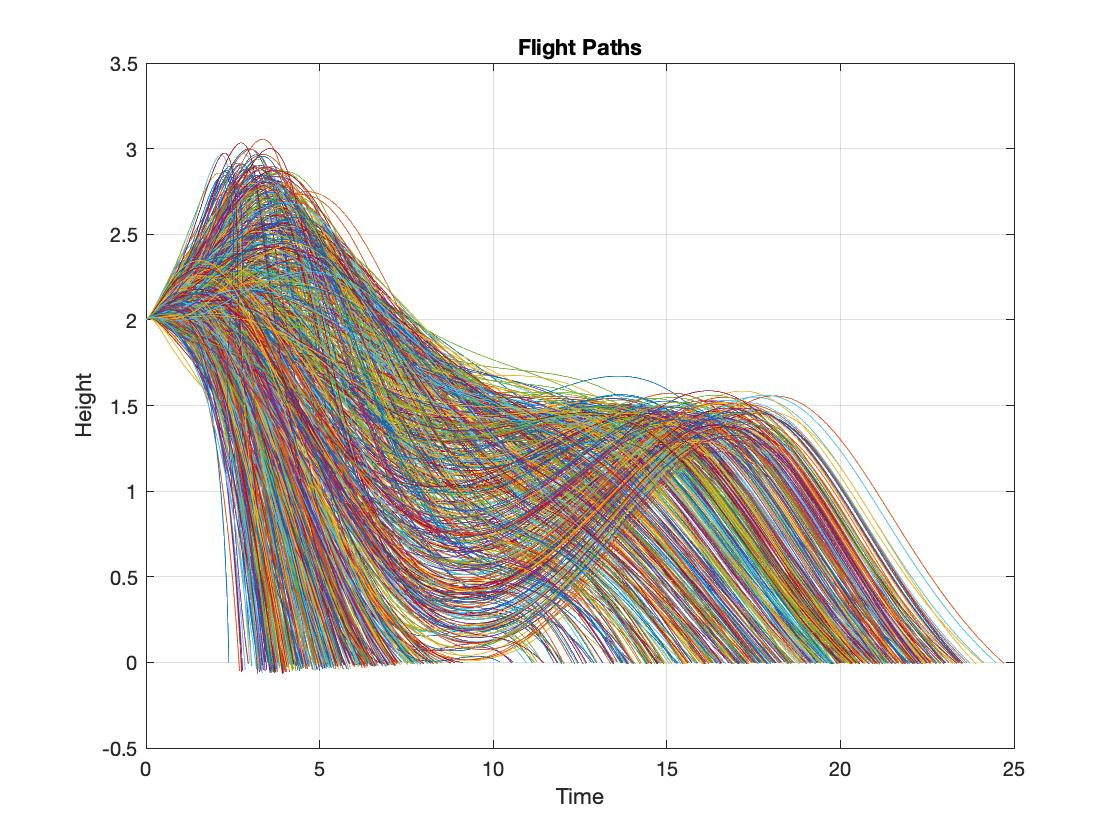
\includegraphics[width=0.6\linewidth]{flight paths.jpg}
	\caption{Flight Paths}
\end{figure}
The mean, median, maximum, and standard deviation are shown below:
\begin{align*}
    x_{max} &= max(x) = 24.7039 m\\
    \bar{x} &= mean(x) = 13.4204 m\\
    x_{median} &= median(x) = 15.4316 m\\
    \sigma &= std(x) = 6.95\\
\end{align*}

Plotting a histogram of my results, shows:
\begin{figure}[H]
	\centering
	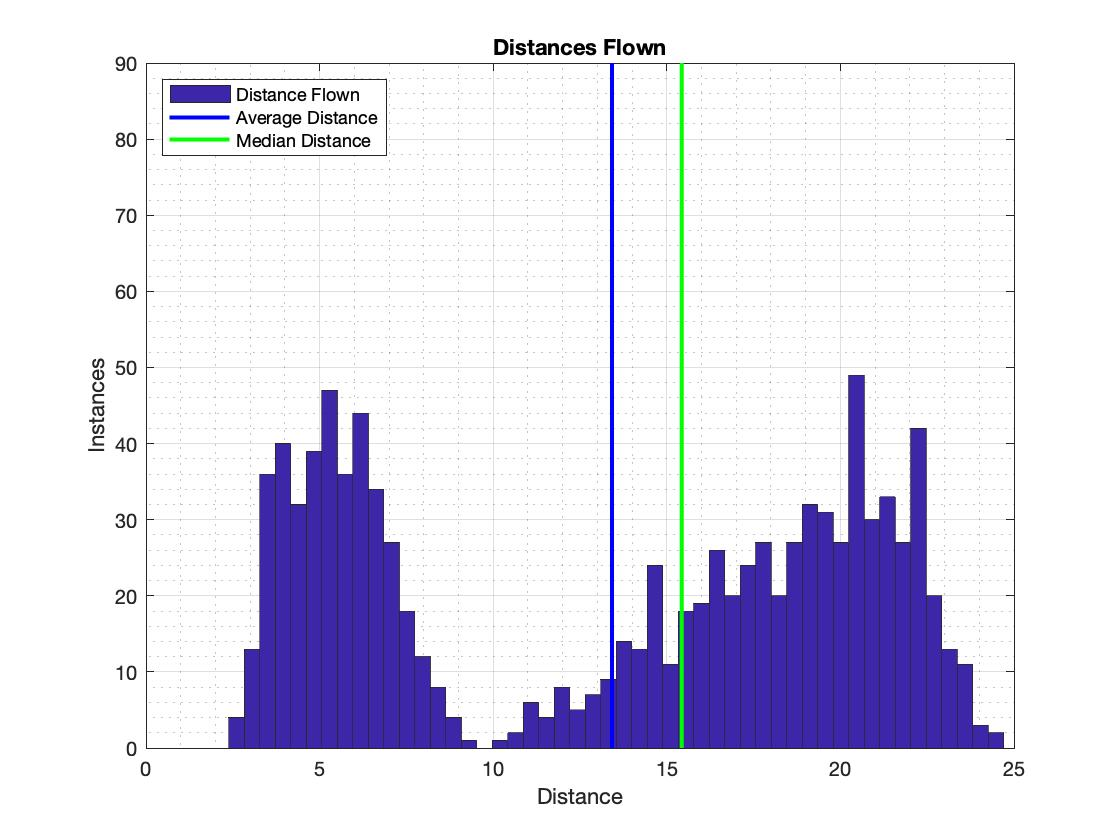
\includegraphics[width=0.6\linewidth]{distances.jpg}
	\caption{Flight Distances' Histogram}
\end{figure}
We can see that our controller was successful and verified the requirements set for it as it averaged a flight distance of 13.42 meters. Since my standard deviation is 6.95 we can say that around 68\% of the time, the glider would land in between 10 to 20 meters.\\
If I eliminate all the nose dives done by my glider, the mean, median, and standard deviation would change. These are the main instances where my initial state guesses were off, not allowing m controller time to stabilize in time. The histogram then looks like:
\begin{figure}[H]
	\centering
	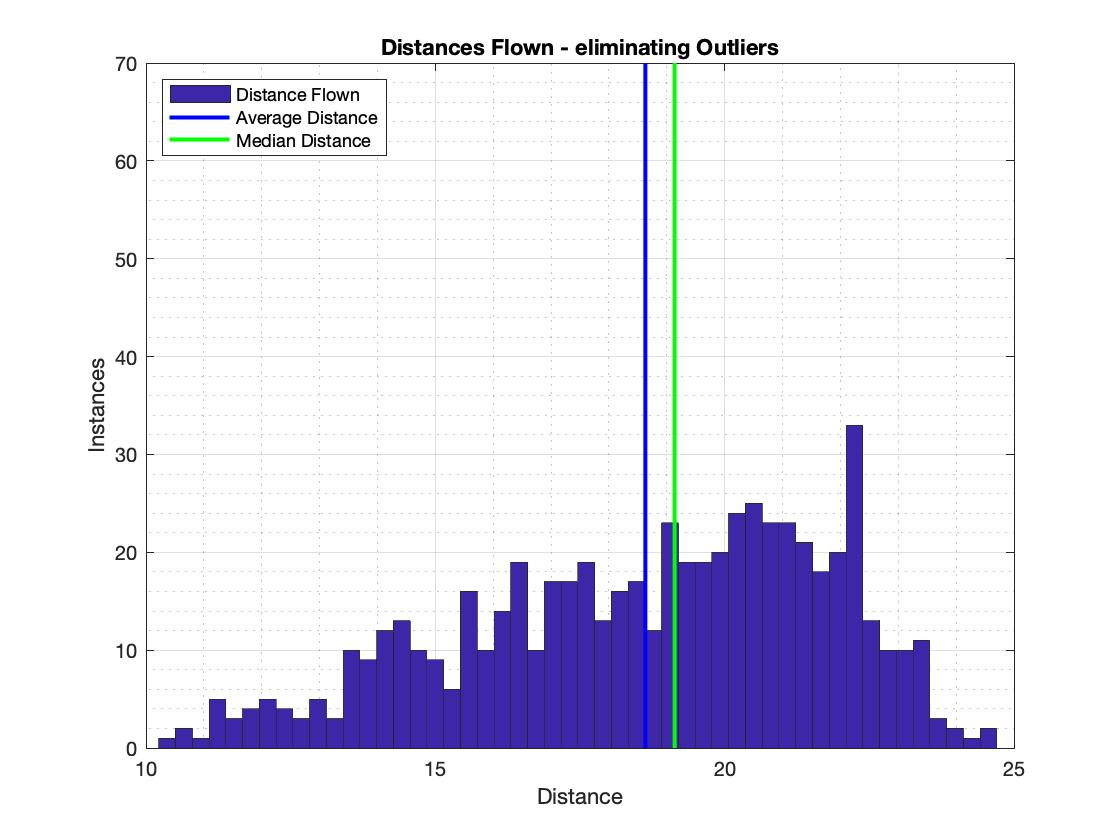
\includegraphics[width=0.6\linewidth]{Distances without outliers.jpg}
	\caption{Flight Distances without Nose-Dives' Histogram}
\end{figure}
The new mean, median, maximum, and standard deviation are shown below:
\begin{align*}
    x_{new,max} &= max(x) = 24.7039 m\\
    \bar{x}_{new} &= mean(x) = 18.6288 m\\
    x_{new,median} &= median(x) = 19.1350 m\\
    \sigma_{new} &= std(x) = 3.1320\\
\end{align*}
\section{Discussion of Results}
After playing around with $Q_{c},R_{c},Q_{o}, and R_{o}$, I was able to get a relatively consistent system. I was mostly able to remove most of the nose dives that produced a binomial distribution. However, my average was about 13.42 meters. The launch angle that worked best with my controller was 10$^{\circ}$, and the elevator length that worked best was 0.2 meters. After a lot of trial and error, I received an output that I was satisfied with. However, this showed that my controller was unable to correct itself enough, showing how my initial guesses were off. This is why we see the instances of a normal distribution regarding the low values, and this is why my standard deviation was high, which I expected. Tough I was able to improve the nature of the consistency of the glide distance, I was unable to produce a flight distance that was further than the record in this class. The outputs showed the limitations to my controller, and if more time was spent on playing around with observer matrices and cost matrices, I could have produced even better results. However, that meant trying millions of combinations, which would have been manually impossible. Therefore, if I were to improve this next time, I would try to build an optimizing function, that would allow me to compute for the best observer and cost matrices, to efficiently glide my glider, and produce the best output.

\section{Acknowledgements}

$\begin{bmatrix}
1
\end{bmatrix}$ Melkior Ornik: Provided the DesignProblem03 files, from which the code was extracted to find the equations of motions, equilibrium values, and run the controller. \\
\\
$\begin{bmatrix}
2
\end{bmatrix}$ Pranay Thangeda: Provided feedback on my thought process around finding my K and L matrices, and guided me around how to play around with 
$Q_{c},R_{c},Q_{o},R_{o}$. \\
\\
$\begin{bmatrix}
3
\end{bmatrix}$ Ben Schultz: Helped me out with general questions, and was a great work buddy. He motivated me to stay on task, and made sure I was grinding through. Would not have been able to sit through all those trial runs whilst playing around with my observer and cost matrices without him.

\end{document}
